
\section{\textit{ConTEB} Details}\label{app:conteb_stats}

% \begin{figure*}[htbp]
%   \centering
%   \includegraphics[width=\textwidth]{images/benchmark_creation_horizontal.pdf}
%   \caption{Benchmark creation process.}
%   \label{fig:benchmark_creation}
% \end{figure*}



This appendix describes the data generation process employed in this project. The methodology varies based on the dataset source, but generally, long documents are segmented into smaller chunks. If preexisting queries are available, they are mapped to relevant chunks using either provided answer spans (e.g., SQuAD) or tagged using GPT-4o. In cases where queries are unavailable, a large language model (LLM) generates them before associating them with the relevant text segments. This approach, illustrated in \ref{fig:benchmark_creation}, is systematically applied across multiple datasets.


\subsection{Wiki-based Datasets} \label{app:wiki-based}

\emph{Football} and Geography are our two wiki-based datasets, focusing on the Sports and Geography domains.

\noindent\textbf{Wikipedia Data Extraction}
The pipeline first retrieves Wikipedia summaries for a given person using the \texttt{wikipediaapi} library. The extracted summary is then split into paragraphs.

\noindent\textbf{Text Rephrasing}
Each paragraph from the Wikipedia summary undergoes a rephrasing process to remove direct mentions of the person’s name while maintaining the original context. The rephrased text replaces names with pronouns such as ‘he’ or ‘she’. This transformation is performed using the GPT-4o model via the following prompt:

\begin{quote}
\textit{
Here is a Wikipedia article:
\texttt{[Full Wikipedia Summary]}
Can you rephrase the following paragraph to remove all mention of the name of the person the article is about? You can leave other names as is and can replace the name with words such as 'he/she' or other generic paraphrases.
\texttt{[Paragraph to be rephrased]}
}
\end{quote}

\noindent\textbf{Question Generation}
For each paragraph in the summary, the model generates three questions related to the person. The questions explicitly mention the person's name but do not include other named entities such as dates or proper nouns. The generation follows this structured prompt:

\begin{quote}
\textit{
Here is a Wikipedia article:}

\texttt{[Full Wikipedia Summary]}

Using specifically the following paragraph, can you ask 3 questions related to the person the article is about? Each question must mention the name of the person, but the question should not contain other named entities (dates, other proper nouns). Format the response as a Python list of strings and do not output anything else.

\texttt{[Paragraph to be used for question generation]}

\end{quote}


\subsection{NarrativeQA, COVID-QA, MLDR}

\textit{NarrativeQA} (literature), \textit{MLDR} (encyclopedic) and \textit{Covid-QA} (medical) consist of long documents, associated to existing sets of question-answer pairs. 

We chunk these documents, and use GPT-4o to annotate which chunk, among the gold document, best contains information needed to answer the query. Since chunking is done \textit{a posteriori} without considering the questions, chunks are not always self-contained and eliciting document-wide context can help build meaningful representations. 

\textbf{Synthetic Query Generation:} To extend MLDR for our training dataset, OpenAI's GPT-4o model is prompted to generate 20-50 realistic queries per document, ensuring that each query aligns with the content of at least one chunk. This is on top of the queries that are already incuded in the dataset. Synthetic queries are included only in our training dataset.


\subsection{Insurance} 
\textit{Insurance} is composed of a long document with insurance-related statistics for each country of the European Union. Countries are often not referred to in-text, but only once in the section title. Therefore, certain chunks require knowledge of their position within the document to be properly disambiguated from others. Questions are manually crafted to require structural understanding for accurate chunk matching. This process, in addition to manual verification of the contextuality quality, makes \textit{Insurance} a controlled dataset. Since questions are crafted after the chunking process, the annotation results directly from the manual question generation process.

\subsection{SQuAD}

\textit{SQuAD} is an extractive QA dataset with questions associated to passages and annotated answer spans, that allow us to chunk individual passages into shorter sequences while preserving the original annotation.

\subsection{ESG Reports}

\textit{ESG Reports} contains long documents from the fast-food industry, with manually annotated query-page pairs from the ViDoRe Benchmark v2 \sidecite{macé2025vidorebenchmarkv2raising}, originally thought for visual retrieving\footnote{\url{https://huggingface.co/datasets/vidore/restaurant_esg_reports_beir}}. We convert all documents to text, chunk them, and re-annotate the resulting passages by hand, filtering out queries that relied solely on visual aspects (e.g., tables, graphs).


% \begin{table*}[h]
%     \centering
%     \small
%     \resizebox{\textwidth}{!}{
%     \begin{tabular}{lcccccc}
%     \toprule
%      & \# Positives (per query) & \# Docs & Tokens/Chunk & Chunks/Doc & Query generation & Chunk Annotation \\
%     \midrule
%     \textbf{In Domain} & \\
%     Chunked MLDR & 100 (1) & 100 & 170.5 & 15.4 & Synthetic & Synthetic \\
%     NarrativeQA & 8575 (1) & 355 & 154.5 & 4.9 & Human & Synthetic \\
%     SQuAD Chunked & 2067 (1) & 2067 & 19.1 & 8.5 & Human & Manual \\
%     \midrule
%     \textbf{Out-Of-Domain} & \\
%     \textcolor{navyblue}{\textbf{Footballers}} & 1767 (1) & 224 & 86.1 & 3.6 & Synthetic & Human in the loop \\
%     \textcolor{navyblue}{\textbf{Geography}} & 5283 (1) & 530 & 113.6 & 4.3 & Synthetic & Human in the loop \\
%     \textcolor{navyblue}{\textbf{Insurance}} & 120 (1) & 1 & 80.7 & 60 & Human & Manual \\
%     Covid-QA & 1111 (1) & 115 & 153.9 & 29.1 & Human & Synthetic \\
%     ESG Reports & 75 (2.3) & -- & -- & -- & Human & Manual \\
%     NanoBEIR* & 650 (1) & 4363.3 & 199.4 & 1 & Human & Manual \\
%     \bottomrule
%     \end{tabular}
%     }
%     \caption{Merged \emph{ConTEB} dataset details and statistics. Controlled datasets are highlighted in \textcolor{navyblue}{\textbf{bold blue}}. Values marked \texttt{--} indicate missing statistics in the source tables.}
%     \label{table:merged_conteb}
% \end{table*}


\subsection{Training Data Statistics}\label{app:training_data}

\autoref{table:training-data} displays information about the training data. Our refined version of MLDR forms a large part of the training corpus. We can see that the majority of chunks are used as positives at least once, ensuring that the model is not biased towards the position of the chunk in the sequence.

\begin{table}[ht]
    \centering
    % \renewcommand{\arraystretch}{1.2} % Adjust row spacing
    \resizebox{\linewidth}{!}{%
    \begin{tabular}{l|rrr|r}
    \toprule
     & MLDR & NarrativeQA & SQuAD & Total \\
    \midrule
    Number of Docs & 8467 & 972 & 442 & 9881 \\
    Number of Chunks & 213001 & 5219 & 14367 & 232587 \\
    Number of Queries & 211933 & 27953 & 67355 & 307241 \\
    Number of Chunks per Doc & 25.2 & 5.4 & 32.5 & 23.5 \\
    \% Chunks with associated Query & 94.6\% & 81.9\% & 100.0\% & 94.61\% \\
    Number of Tokens per Doc & 3962.6 & 819.1 & 4966.1 & 3698.2 \\
    Number of Tokens per Query & 16.7 & 21.9 & 12.5 & 16.3 \\
    \bottomrule
    
    \end{tabular}
    }
    
    \caption[Training dataset statistics]{Training Dataset Statistics} 
    \label{table:training-data}
\end{table}





%\section{Training Setup}\label{app:training_setup}

%We train all our models using a customized version of the \texttt{sentence-transformers} trainer \footnote{\url{https://sbert.net/docs/package_reference/sentence_transformer/trainer.html}}, using the PyTorch BF16  mixed precision on 4-GPU nodes. We use a cosine decay learning rate scheduler with a warm-up phase of 55 steps. Below are the model-specific parameters. All parameters that are not specified are set to the default values of the \texttt{sentence-transformers} trainer. The models are evaluated every 100 training steps.

%\subsection{ModernBERT base variants}
%We fine-tune \texttt{modernbert-embed-base} and \texttt{gte-modernbert-base} using a per-device batch size of 8 and a learning rate of $1e-4$.

%\subsection{ModernBERT large}
%We fine-tune \texttt{modernbert-embed-large} using a per-device batch size of 4 and a learning rate decreased accordingly to $5e-5$.

% \subsection{Prefix}


\section{Implementation Details}

\subsection{Sequence prefixes}

ModernBERT-based models are trained with query and document prefixes. We apply the same approach in our training and inference frameworks. After several tests, we opt for using a single document prefix for the Late Chunking sequence, instead of adding a document prefix at the beginning of each chunk inside the same sequence. We separate chunks with [SEP] tokens to let the model understand the concept of chunks during its token embedding computation.


\subsection{Late Interaction Models}

We leverage the \texttt{pylate} \sidecite{PyLate} library for the Late Interaction implementation. For training LI models with InSeNT, we adapt the LI mechanisms to incorporate it with Late Chunking in our own codebase. In particular, we do not use token skiplists at inference time, and use a single document prefix for the whole document sequence.

\section{Additional Results}
\label{app:res}

\subsection{Training with concatenated short documents}

Results of training an InSeNT model with concatenated short document data (using the Nomic dataset) are available in \autoref{table:nomic-results}. Short docs are clustered from the \texttt{nomic-supervised} dataset \cite{nussbaum2024nomic} following \sidecite{morris2024contextualdocumentembeddings}. This approach did not yield promising results, proving that natively long documents are necessary to induce relevant in-sequence signal.


\begin{table*}[ht]
    \centering
    \renewcommand{\arraystretch}{1.2} % Adjust row spacing
    \resizebox{\textwidth}{!}{%
    \begin{tabular}{l|rrr|rrrr|r|rr}
\toprule
     & MLDR & SQuAD & NarrativeQA & Football & Geography & COVID-QA & Insurance & NanoBEIR & Average & Runtime (s) \\
    \midrule
    MB & 78.4 & 73.4 & 77.9 & 19.1 & 56.2 & \textbf{61.7} & 12.4 & \textbf{63.2} & 55.3 & 40.0\\
    \midrule
    MB+InSeNT(Nomic) & 77.8 & 76.0 & 76.2 & 26.2 & 62.7 & 38.8 & 63.7 & 59.9 & 60.2 & 36.3\\
    MB+Late Chunking & 78.5 & 77.1 & 75.8 & 54.6 & 89.6 & 40.0 & 41.0 & \textbf{63.2} & 65.0 & 36.3 \\
    \textbf{Ours: MB+InSeNT} & \textbf{88.7} & \textbf{80.9} & \textbf{81.3} & \textbf{63.9} & \textbf{90.7} & 56.0 & \textbf{100.0} & 60.4 & \textbf{77.8} & 36.3 \\
    \bottomrule
    \end{tabular}}

    \caption[ConTEB evaluation results]{Evaluation (nDCG@10) of baseline models and our proposed method on \textit{ConTEB}. We show MB+InSeNT(Nomic) behaves like a non-contextual model after training on independant documents concatenated in a single sequence.} 
    \label{table:nomic-results}
\end{table*}

\subsection{Full ablation results on $\lambda_{seq}$}

We show the results of the different values for $\lambda_{seq}$ on all our evaluation sets.

% \begin{figure*}
%     \centering
%     \includegraphics[width = 1\linewidth]{images/lambda_seq_mb-large_full.pdf}
%     \caption{Evaluation results for varying $\lambda_{seq}$ values with ModernBERT-Large. Trends vary across the datasets depending on their nature.}
%     \label{fig:lambda_seq_mb_appendix}
% \end{figure*}

% \begin{figure*}
%     \centering
%     \includegraphics[width = 1\linewidth]{images/lambda_seq_colbert_full.pdf}
%     \caption{Evaluation results for varying $\lambda_{seq}$ values with GTE-ModernColBERT. Trends vary across the datasets depending on their nature.}
%     \label{fig:lambda_seq_colbert_appendix}
% \end{figure*}

\begin{figure*}
    \centering
    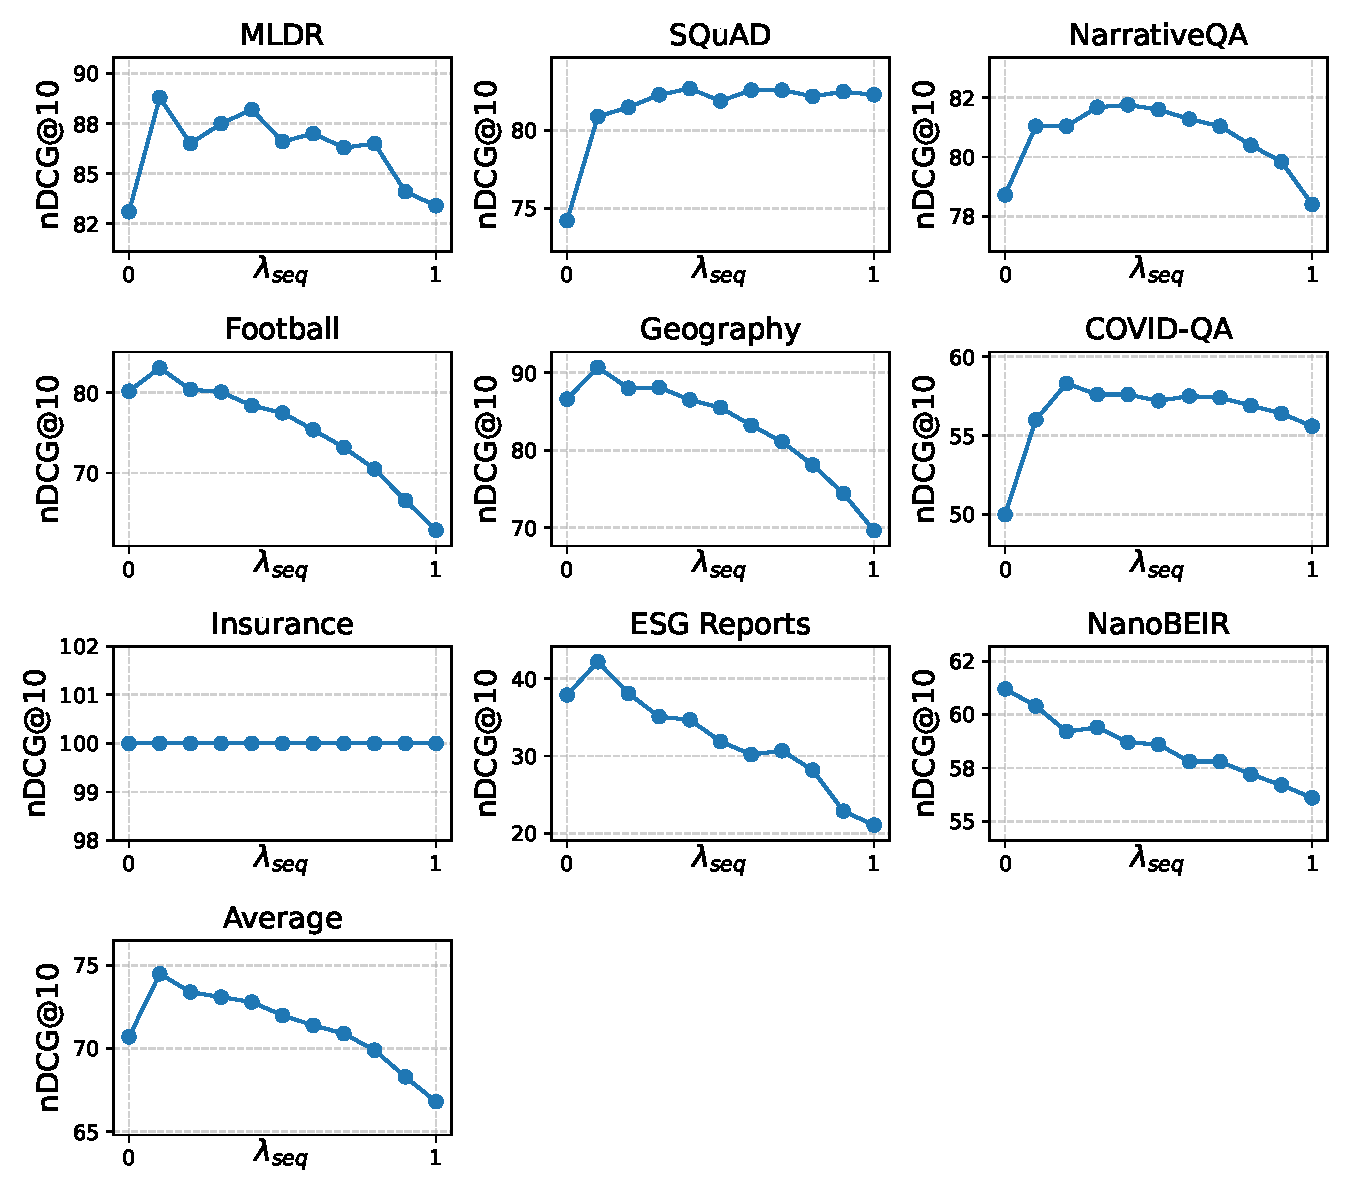
\includegraphics[width=0.49\linewidth]{images/conteb_images/lambda_seq_mb-large_full.pdf}
    \hfill
    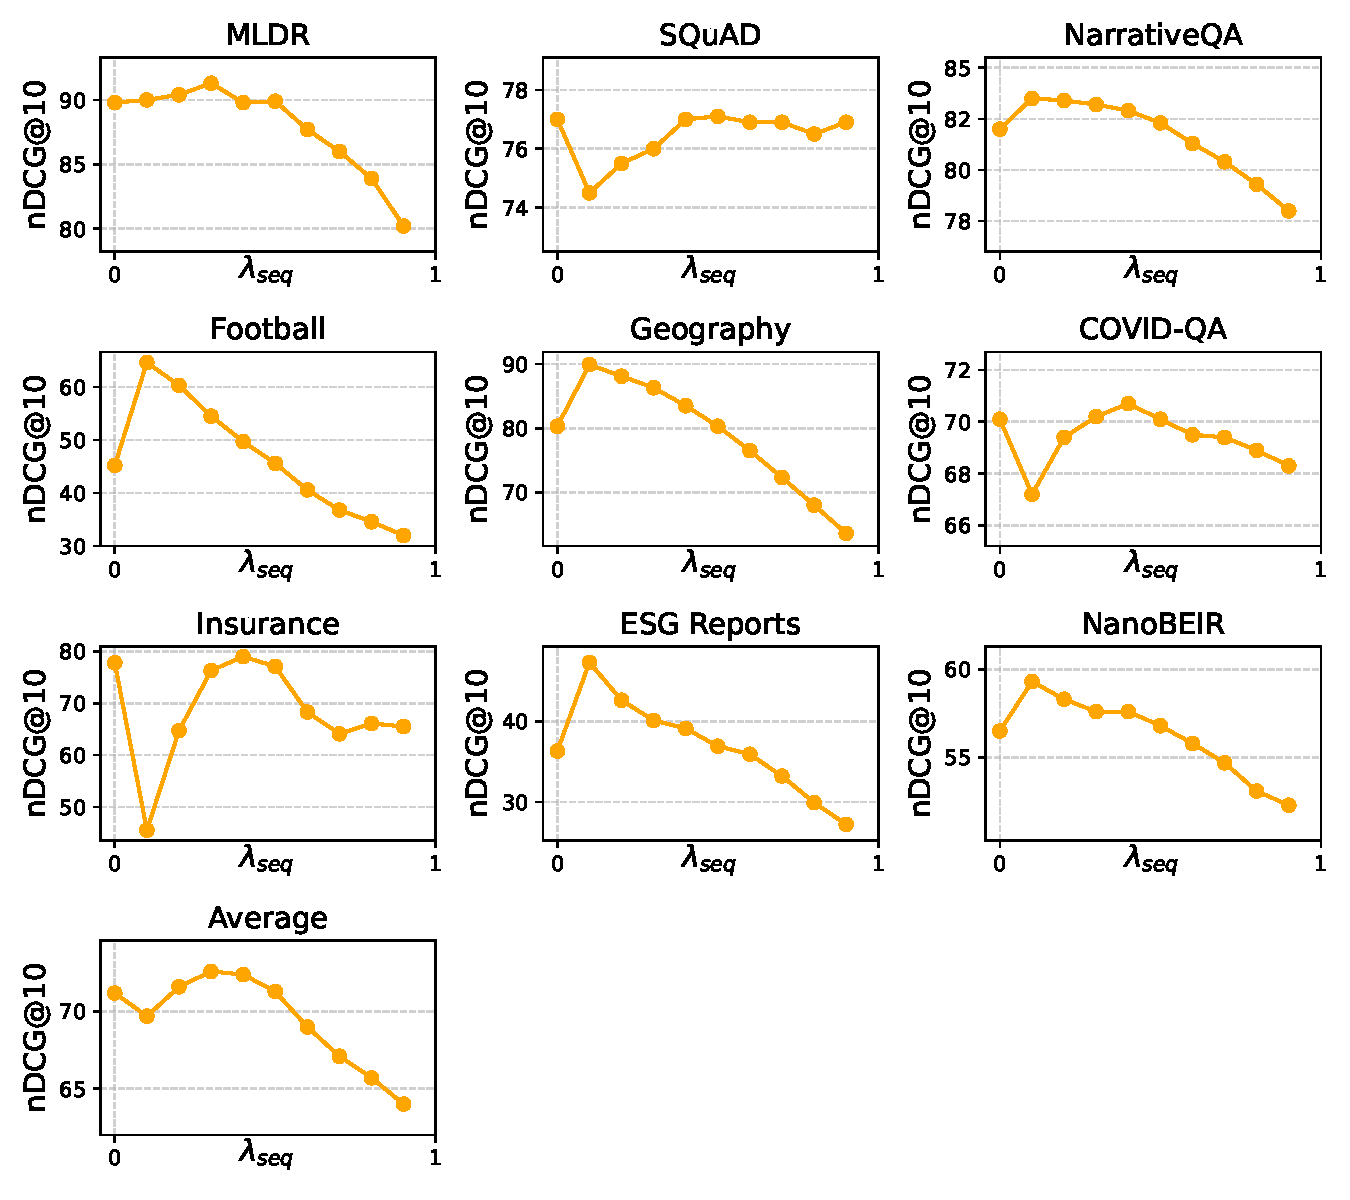
\includegraphics[width=0.49\linewidth]{images/conteb_images/lambda_seq_colbert_full.pdf}
    \caption[$\lambda_{seq}$ evaluation results]{Evaluation results for varying $\lambda_{seq}$ values. Left: ModernBERT-Large. Right: GTE-ModernColBERT. Trends vary across the datasets depending on their nature.}
    \label{fig:lambda_seq_side_by_side}
\end{figure*}

\subsection{Extending context beyond 8192 tokens}

ModernBERT was trained on documents of up to 8192 tokens \sidecite{modernbert}. Its Late Interaction counterpart, GTE-ModernColBERT, was exclusively fine-tuned on documents of no more than 300 tokens. However, its generalization capabilities to longer documents have been shown by its developers \sidecite{GTE-ModernColBERT}, hinting at the fact that further research along those lines could be tried for both the bi-encoder and the LI variants.

Based on these results, we tried two approaches to handle documents longer than 8192 tokens with ModernBERT (necessary for the ESG reports dataset): computing Late Chunking with a context of max. 8192 tokens in an sliding window fashion (computing chunk embeddings in several forward passes of 8192 tokens, with 10 overlapping chunks between the various windows), and naively feeding the complete documents to the embedder. 

To our surprise, the latter worked better by a large margin (43.1 on ESG as reported in \ref{table:results}, vs 25.4 for the sliding window approach), so we reported the results of this approach. Further studies could be led to better understand the dynamics underlying this extension.
